\handsonEnv
%%%
\begin{frame}
\frametitle{\href{https://wci.llnl.gov/simulation/computer-codes/visit/}{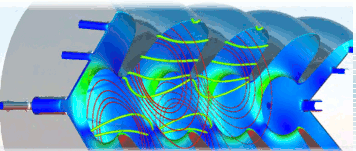
\includegraphics[height=.85cm]{figs/visit-logos/VisIt-02}} \hspace{-.85cm}{\bf \textcolor{lightgray}{VisIt}}: Intermesso ii}

\vspace{-1mm}
\begin{beamerboxesrounded}[upper=block head,lower=block body,shadow=true]{\bf Hands-on...}%Assignment ii}
%        \textcolor{DarkRed}{\ding{231}} try loading some of the datasets we used with ParaView [{\small \textcolor{gray}{\tt headsq.vtk}, \textcolor{gray}{\tt testRectilinearGrid.vtk}, \textcolor{gray}{\tt disk\_out\_ref.ex2}, ...}] --or-- your own data!!!
        \textcolor{DarkGreen}{\ding{231}} Using the 
                {\small ``\textcolor{gray}{\texttt{aneurysm}}''} dataset
                --or-- \textit{your own data},
		generate a time sequence movie

	\pause
        \textcolor{DarkGreen}{\ding{231}} Experiment with keyframming, lighting, ... or any of the other techniques we have been discussing

\end{beamerboxesrounded}

\pause
\vspace{.75mm}
\begin{columns}
\begin{column}{5cm}
	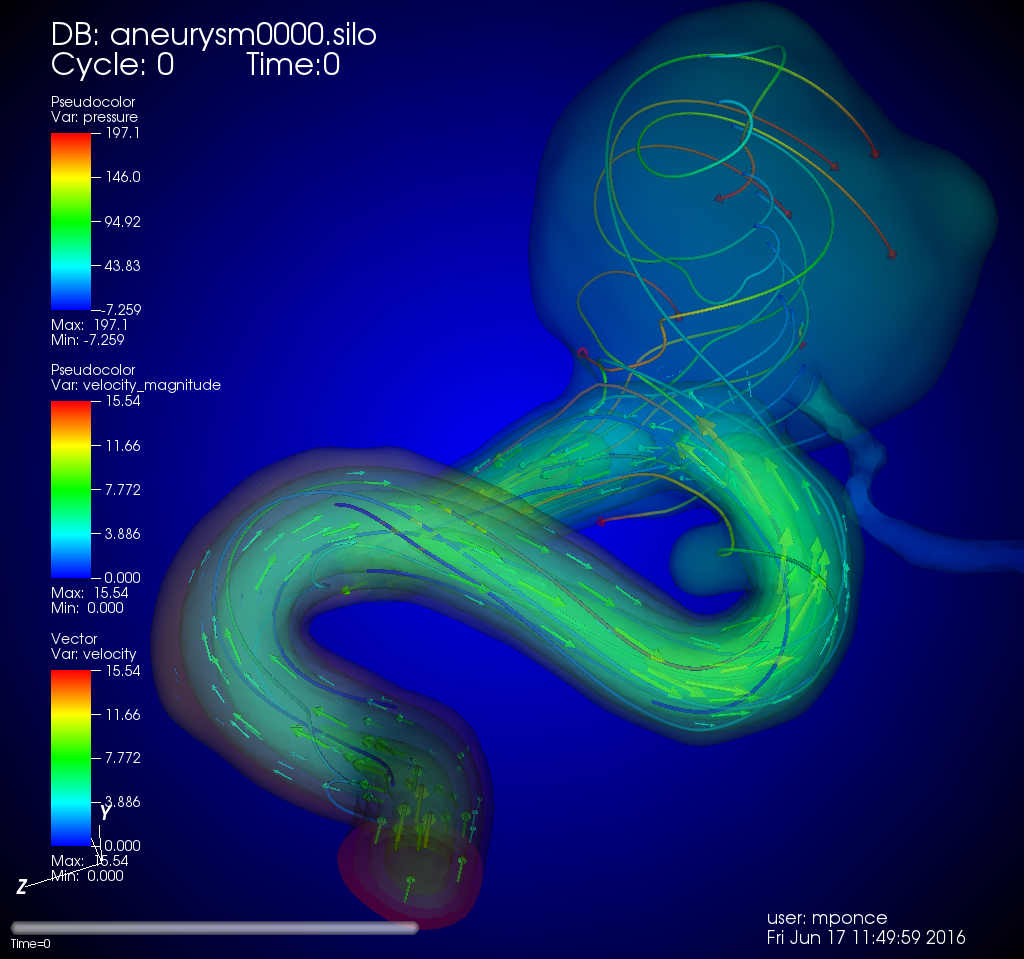
\includegraphics[width=\columnwidth]{figs/visit-pract/VisIt_aneurysm0}
\end{column}
\begin{column}{6cm}
	\includemovie[repeat=5]{.8\columnwidth}{.8\columnwidth}{figs/movies/aneurism_movie1.mp4}
\end{column}
\end{columns}

\pause
\begin{columns}
\begin{column}{12cm}
\vspace{-.5mm}
{\tiny\bf
More info about this dataset at: \\
\vspace{-2.5mm}
\url{http://www.visitusers.org/index.php?title=Blood_Flow_Aneurysm_Tutorial_Dataset_Exploration}
}
\end{column}
\end{columns}
\end{frame}
%%%
\resetEnv
\basicEnv
